\documentclass[conference]{IEEEtran}

% *** CITATION PACKAGES ***
\usepackage{cite}

% *** GRAPHICS RELATED PACKAGES ***
\ifCLASSINFOpdf
\usepackage[pdftex]{graphicx}
\usepackage{tikz}
\usepackage{caption}
\usepackage{subfig}

% *** MATH PACKAGES ***
\usepackage[cmex10]{amsmath}

% *** SPECIALIZED LIST PACKAGES ***
\usepackage{algorithmic}

% correct bad hyphenation here
\hyphenation{op-tical net-works semi-conduc-tor}

\begin{document}
  \title{Fast Target Link Flooding Attack Detection Scheme \\by Analyzing Traceroute Packets Flow}

  \author{
    \IEEEauthorblockN{Takayuki Hirayama, Kentaroh Toyoda, and Iwao Sasase}
    \IEEEauthorblockA{Dept. of Information and Computer Science, Keio University\\
    3-14-1 Hiyoshi, Kohoku, Yokohama, Kanagawa, 223-8522 Japan, \\
    Email: hirayama@sasase.ics.keio.ac.jp}
  }

  \maketitle

  \begin{abstract}
    Recently, a botnet based DDoS (Distributed Denial of Service) attack, called target link flooding attack, has been reported that cuts off specific links over the Internet and disconnects a specific region from other regions.
    Detecting or mitigating the target link flooding attack is more difficult than legacy DDoS attack techniques, since attacking flows do not reach the target region. 
    Although many mitigation schemes are proposed, they detect the attack after it occurs.
    In this paper, we propose a fast target link flooding attack detection scheme by leveraging the fact that the traceroute packets are increased before the attack caused by the attacker's reconnaissance.
    Moreover, by analyzing the characteristic of the target link flooding attack that the number of traceroute packets simultaneously increases in various regions over the network, we propose a detection scheme with multiple detection servers to eliminate false alarms caused by sudden increase of traceroute packets sent by legitimate users.
    We show the effectiveness of our scheme by the computer simulation.
  \end{abstract}

  \IEEEpeerreviewmaketitle

  \section{Introduction}\label{Sec:Introduction}
    It is an urgent demand to avoid attacking against key network infrastructures, e.g., government servers, smart grid system, banking system, or power plant system.
    Recently Kang et al. propose a bot-based DDoS (Distributed Denial of Service) attack \cite{Crossfire}. The link flooding attack cuts off specific links over the Internet and disconnects a specific region from other regions.
    It uses botnet and public servers to flood the specific links.
    The attack has two main features: 1) attacking flows do not directly reach the target area and 2) each bot communicates with public servers with a valid IP address and transmits low-rate traffic.
    Therefore many conventional DDoS detection or mitigation schemes, e.g., \cite{ddossurvey01, ddossurvey02}, are ineffective against the target link flooding attack.

    Some attack detection or mitigation schemes against the target link flooding attack are discussed in industrial and academia.
    For example, Lee et al. propose an AS (Autonomous System) level target link flooding attack avoidance scheme \cite{CoDef}.
    Gkounis proposes a cross-domain DoS link-flooding attack detection and mitigation scheme which using SDN (Software Defined Networking) \cite{crossdomain}.
    Xue et al. propose an attack detection scheme based on the characteristics of a congested link such as packet loss rate or RTT (Round Trip Time) \cite{DetectTLFA}.
    However all of the above schemes work after a link congestion occurs and they cannot detect the attack before it occurs because they use characteristics of congested links or the router's link failure detection mechanism.
    Therefore, the target area remains to be cut off from the Internet until a detection scheme recovers destructive links.
    This delay is fatal for specific system such as a power supply system or a financial service.
    Hence, it is an urgent demand to detect an attack before link congestion occurs.
   
    In this paper, we propose a fast target link flooding attack detection scheme by using the fact that the traceroute packets are increased before the attack occurs.
    Attackers should send many traceroute packets before the target link flooding attack since they should investigate the target links that must be flooded.
    Hence our scheme lets each router (or AS) count the number of traceroute packets that pass through it and leverages a change point detection algorithm to detect a point that suddenly the number of traceroute packets increases.
    Moreover we exploit that the number of traceroute packets simultaneously increases in various regions over the network.
    We use the combination of detection servers located across the network to capture the characteristic of the attack and eliminate false alarms caused by sudden increase of traceroute packets sent by legitimate users.
    Our scheme has following features:
    1) To our knowledge, this is the first work that can detect the target link flooding attack before a link congestion occurs.
    This feature helps other mitigation schemes and gives time to prepare for the attack.
    2) Our scheme uses only the number of traceroute packets and thus it is easy to distinguish the target link flooding attack from normal link congestions and normal link failures since a behaviour of increase of traceroute packets is independent of a link congestion and a link failure.
    In order to show the effectiveness of our scheme, we evaluate the detection accuracy with a real Internet topology called Caida AS Relationships Dataset \cite{as-relation}.

    The rest of this paper is structured as follows: Section \ref{Sec:Preliminaries} describes the AS level network and the model of the attacker.
    Related work is described in Section \ref{Sec:Related Work}.
    The proposed scheme is described in Section \ref{Sec:Proposed Scheme}.
    Simulation results and evaluation are discussed in Section \ref{Sec:Evaluation}.
    Finally we conclude our discussion in Section \ref{Sec:Conclusion}.

  \section{Preliminaries}\label{Sec:Preliminaries}
  \subsection{Relationships between Autonomous Systems}\label{Sec:Relationships between Autonomous Systems}
    An AS (Autonomous System) is a network managed by a single administrative domain e.g., Internet service providers (ISPs), companies and universities and an AS consists of routers and links.
    The Internet consists of thousands of ASes and connections between ASes keep global connectivity.
    According to \cite{as-relation, AS1, AS2}, the network between ASes has hierarchical structure and scale-free characteristics.
    Relationships between ASes can be roughly classified into provider-customer connection, peer-to-peer connection, and sibling connection.
    A provider-customer connection connects two ASes 1) a provider AS who sells global connectivity and 2) a customer AS who pays for the full route information of the Internet.
    A peer-to-peer connection connects equal ASes, e.g., between same scale customer ASes.
    A sibling connection connects two small ASes to enhance connectivity or for backup connectivity.
    ASes located on the top of hierarchy are called Tier1 and connect to vast numbers of customer ASes.

  \subsection{Attacker Model}\label{Sec:Attacker Model}
    Here, we describe the steps of the target link flooding attack.
    The attacker uses PPI (Pay-Per Install) services to prepare bots.
    PPI offers servers and executes any program that a user specifies on them.
    Therefore the attacker has ability to run any program and command on the bots.
    \figurename~\ref{The schema of the target link flooding attack} illustrates the schema of target link flooding attack.
    The attacker's goal is to disconnect a specific region called target area from other regions.
    For this goal, the attacker takes the following procedures.

    First the attacker selects two sets of public servers, which are the target servers and the decoy servers.
    The target servers are located in the target area while the decoy servers are located around the target area.
    The attacker has no information about a location of bots over the Internet.
    Therefore the attacker creates a map of network topology using bots and target servers before the attack.
    To create the map, each bot runs traceroute commands to target servers and finds paths from the bot to target servers.
    When all bots complete to find the paths, the attacker aggregates all traceroute results and finds target links which frequently appear in the results.
    Then the attacker selects bot-decoy pairs which flood the target links.
    To select the pairs, each bot runs traceroute commands to decoy servers and finds the paths which contain the target links.
    Once the attacker selects target links and bot-decoy pairs, the attacker sends a command to make bots send low-rate traffic.
    As a result, even if the attack flows between bots and decoy servers only flood the target links, the target area is isolated from the outer region.
    \begin{figure}[!t]
      \centering
      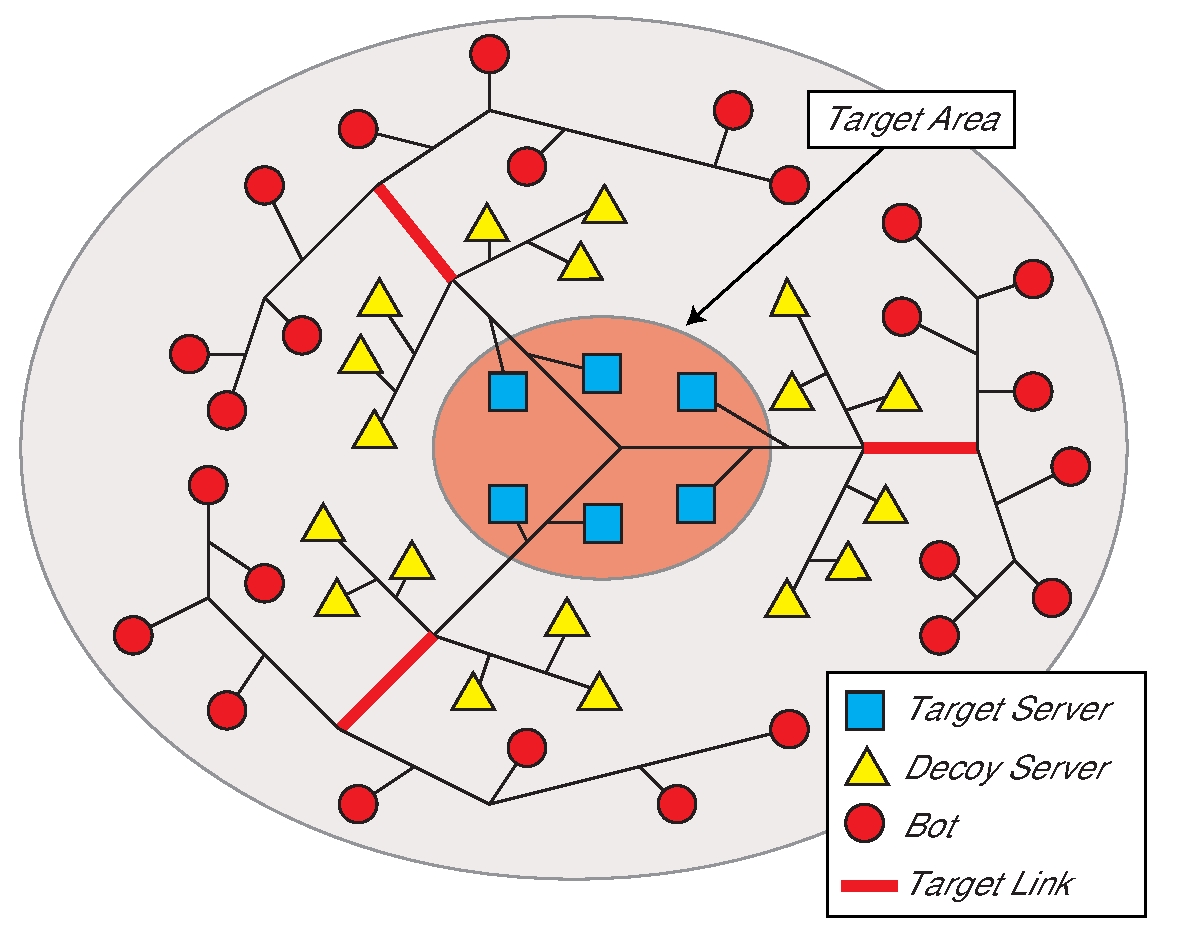
\includegraphics[clip, width=2.8in]{./image/Elements.eps}
      \caption{The schema of the target link flooding attack.}
      \label{The schema of the target link flooding attack}
    \end{figure}

  \section{Related Work}\label{Sec:Related Work}
    There are many researches to detect and mitigate network layer distributed denial-of-service (DDoS) attacks \cite{ddossurvey01, ddossurvey02}.
    However detection schemes against network layer DDoS attacks cannot effect against botnet-driven DDoS attacks since the attacking flow seems to be legitimate e.g., using valid IP addresses or transmitting low-rate traffic.

    Lee et al. \cite{CoDef} propose CoDef (Collaborative Defence) which is an AS (Autonomous System) level target link flooding attack avoidance scheme.
    When target link flooding attack occurs, a congested router sends a rerouting request and a rate-control request to source ASes to mitigate a link congestion.
    This is because an attacker must aggregate attack flows to the target link for the success of the attack.
    Moreover the congested router distinguishes legitimate ASes from attacking ones by monitoring the behavior of source ASes.
    As a result, this scheme forces the attacker to make an untenable choice: either conforming to the request and giving up the attack persistence at the target link, or rejecting the requests and obeying the flow control.

    Gkounis \cite{crossdomain} proposes a cross-domain DoS link-flooding attack detection and mitigation scheme which using SDN (Software Defined Networking).
    This scheme detects the attack by monitoring a link congestion.
    When it detects the attack it reroutes flows which pass a congested link to disperse flows.
    Even if the attacker tries to find new target links, the attacker cannot follow rapid reroutings by SDN.
    Therefore each bot must increase attack traffic to fill up the target link.
    However such reaction is suspicious for attackers and the scheme can limit the bandwidth of suspicious flow sources.

    Xue et al. \cite{DetectTLFA} propose an attack detection scheme called LinkScope based on the characteristics of a congested link such as packet loss rate or RTT (Round Trip Time).
    This scheme runs on the end host (e.g., the server in a target area) and does not require the modification of routers.

    Gillani et al. \cite{agile} propose an attack mitigation scheme which reallocates network resources over virtual networks.
    An attacker performs network reconnaissance to select target links before the target link flooding attack and it may take a few minutes.
    Therefore this scheme changes the footprint of critical resources before the attacker's reconnaissance has been completed.
    However this scheme requires to constantly reassign resources even though an attack did not occur.

    The above researches \cite{CoDef,crossdomain,DetectTLFA} can effectively detect the target link flooding attack and mitigate the damage of the attack.
    However they work after a link congestion occurs.
    Therefore the target area remains to be cut off from the Internet until a detection scheme recovers destructive links.
    This delay is fatal for specific system such as a power supply system or a financial service.
    Hence it is an urgent demand to detect an attack before link congestion occurs.

  \section{Proposed Scheme}\label{Sec:Proposed Scheme}
    Here, we propose a fast detection scheme of the target link flooding attack by using the number of traceroute packets observed in each router.
    We focus on the behavior of bots controlled by the attacker.
    In the target link flooding attack, all bots trace paths to the target servers and the decoy servers before the attack.
    As a result of bot's reconnaissance, the total number of traceroute packets must increase compared to a peacetime.
    If a router detects this foretaste, it may be able to detect the attack before occurrence.
    Moreover we only use the number of traceroute packets, our scheme can effectively detect an attack symptom without incurring false alarms.

  \subsection{Algorithm}\label{Sec:Algorithm}
    \begin{figure}[!t]
      \centering
      \includegraphics[clip, width=2.8in]{./image/ProposedScheme_a.eps}
      \caption{A scheme of traceroute log collection.}
      \label{A scheme of traceroute log collection}
    \end{figure}
    Here, we try to detect a target link flooding attack by collecting information from ASes.
    \figurename~\ref{A scheme of traceroute log collection} shows an example how the detection server collects the information of traceroute packets from each router.
    Each AS controls some routers and one detection server.
    Routers are connected to end hosts and forward packets from sources to destinations.
    End hosts are divided into two categories: 1) legitimate users and 2) bots.
    Routers log the information of traceroute packets e.g. timestamp and IP addresses, whenever they process traceroute packets and generate an ICMP Time Exceeded packet.
    Routers transmit the logs to a detection server.
    Then each detection server counts the number of cumulative traceroute packets $c_{t}$.

    As we described before, we want to detect a point that suddenly the number of traceroute packets $c_i$ increases.
    That is, we detect a change point in $C = (c_1, c_2, \cdots, c_t)$ where $t$ denotes the latest time index.
    We leverage a novel change point detection scheme called ChangeFinder \cite{changeFinder} to realize it.
    ChangeFinder detects points that suddenly change in a given time series data.
    It first detects outliers in $C$ by calculating abnormality $a_i$ in each point $c_i$ for $i = [1, t]$ and then detects change points in $(a_1, \cdots, a_t)$ by smoothing $(a_1, \cdots, a_t)$ with the window size $T$.
    The idea behind smoothing is to remove the effect of solo outliers.
    When appropriate $T$ is chosen, only change points are accurately detected.
    Abnormality at point $i$ is defined as the fitness of an observed value $c_i$ against the probability density function $p_{i-1}$ that calculated from $(c_1, \cdots, c_{i-1})$.
    More specifically, each detection server calculates a logarithmic loss score $a_i$ as denoted in the Eq.~(\ref{LossScore}).
    \begin{equation}
      a_i = - \log{p_{i-1}(x = c_i | c_1, \cdots, c_{i-1})},
      \label{LossScore}
    \end{equation}
    where $p_{i-1}(x)$ is the conditional probability density function calculated from $(c_1, \cdots, c_{1-1})$.
    Since we assume the AR (Auto Regression) model for $c_i$, $p_{i-1}(x)$ is denoted as Eq.~(\ref{ARmodel}).
    \begin{equation}
      p_{i-1}(x) = \frac{ 1 }{ \sqrt{ 2\pi } \sigma } \exp{ \left (- \frac{ (x-w)^2 }{ 2\sigma } \right ) },
      \label{ARmodel}
    \end{equation}
    where $\sigma$ denotes a variance of a noise term $\epsilon$ in the AR model and $w$ is denoted as $w = \sum_{j}^{k} \alpha_j (c_{i-j} - \epsilon) - \epsilon$.
    Then, we detect change points in $a_i$ for $i = [1, t]$.
    As we described before, simply detecting high $a_i$ as a change point may bring about the false alarm due to the possibility of an outlier.
    Therefore, we then calculate the $T$-averaged score $\overline{a}_i$ with latest $T$ anomaly values i.e., $(a_{i - T + 1}, \cdots, a_i)$.
    \begin{equation}
      \overline{a}_i = \frac{ 1 }{ T } \sum_{ j = i - T + 1 }^{ i } a_j.
      \label{Smoothing}
    \end{equation}
    We calculate the abnormality of $\overline{a}_i$ with $(\overline{a}_1, \cdots, \overline{a}_{i - 1})$ in the same way of $a_i$ in Eq.~(\ref{LossScore}) and Eq.~(\ref{ARmodel}) and obtain scores $s_i$ for $i \in [1, t]$.

    In the case of the real Internet, not only bots controlled by the attacker but also legitimate users send traceroute packets.
    Thus, traceroute packets sent by legitimate users act as a `noise' from the perspective of the attack detection.
    We suppose random noise which are randomly sent by legitimate uses.
    The scores calculated by ChangeFinder during peacetime vary according to the amount of random noise.
    Therefore we calculate
    \begin{equation}
      d_i = s_i - s_{i-1}
      \label{Difference}
    \end{equation}
    for $i = [2, t]$ and if $d_i$ is higher than the predefined threshold $d_{th}$, a detection server raises an alarm.

    We focus on the fact that the number of traceroute packets simultaneously increases in the near ASes when the link flooding attack occurs.
    Therefore, we use a global detection server \cite{globaldetector} which collects detection results from detection servers located in each AS.
    A concept of global detection server is illustrated in \figurename~\ref{A concept of global detection server}.
    When multiple detection servers, say $N_{th}$ out of $N_{\text{AS}}$ servers, simultaneously raise an alarm, where $N_{\text{AS}}$ indicates the number of AS which has the detection server, we detect an attack.
    \begin{figure}[!t]
      \centering
      \includegraphics[clip, width=2.8in]{./image/GlobalDetector.eps}
      \caption{A concept of global detection server.}
      \label{A concept of global detection server}
    \end{figure}

  \subsection{Discussion}
  \subsubsection{Pros and Cons}
    We discuss the pros and cons of our scheme.
    Our scheme detects the target link flooding attack before a link congestion occurs and gives time to prepare for the attack to other mitigation schemes.
    Moreover, since our scheme uses only the number of traceroute packets, our scheme easily distinguishes normal link congestions from the target link flooding attack.
        
    However our scheme needs the training phase at first to grasp the normal condition of the traceroute packets flow.
    We describe the details of training data at Section \ref{Sec:Evaluation}.

    Our scheme cannot detect the attack if the attacker less frequently sends traceroute packets in order not to be detected by the detection system.
    However such a slow reconnaissance brings several disadvantages to the attacker.
    First, the attacker has to control bots longer time.
    Second, the condition of traced links may change as time goes on.

  \subsubsection{Computational Complexity}
    We discuss the computational complexity of our scheme.
    Our scheme first calculates the number of cumulative traceroute packets within an AS.
    The computational complexity of this summation is $O(N_{Routers})$ where $N_{Routers}$ denotes the number of routers within an AS.
    Then our scheme calculates Eqs.~(\ref{LossScore})-(\ref{Difference}).
    The computational complexity of Eqs.~(\ref{LossScore})-(\ref{Difference}) is constant regardless of the length of $C = (c_1, \cdots, c_t)$, since they use only some latest values to calculate the abnormality.
    Moreover we use the number of cumulative traceroute packets $c_i$ which is one-dimensional time series data as input of ChangeFinder and the number of routers also have no influence.
    The other factors which have an effect on the computational complexity are the order of AR model $k$ and the window size of smoothing $T$.
    Here, we select $k=1$, $T=5$, and computational complexity of ChangeFinder is $O(1)$.
    Finally the computational complexity in Eq.~(\ref{Difference}) is $O(1)$.
    Therefore the biggest factor of computational complexity is to collect traceroute packets from routers within an AS and our scheme can detect the attack in real time.

  \section{Evaluation}\label{Sec:Evaluation}
    We evaluate the detection accuracy of our scheme by the computer simulation.
    We first evaluate the detection accuracy of each detection server and tune the attack classification threshold $d_{th}$ of each detection server.
    Then we evaluate the detection accuracy of global detection server.
    We use TP (True Positive rate), FP (False Positive rate) and AUC (the Area Under an ROC Curve) value to evaluate the detection accuracy.
    TP denotes the ratio of correctly detected traceroute packets by bots and FP denotes the ratio of mistakenly detected traceroute packets by legitimate users.
    The ROC (Receiver Operating Characteristic) curve is a graph which plots TP against FP sliding the threshold of classification algorithm.
    If an algorithm randomly classifies time series data which includes traceroute packets by bots and one which only includes traceroute packets by legitimate users, the ROC curve indicates the line whose slope is 1.
    The AUC value indicates accuracy of a classification algorithm.
    If an algorithm perfectly classifies a data which includes the attack and one which does not include the attack, the AUC indicates 1.0.
    On the other hand, if an algorithm randomly classifies a given data, the AUC indicates 0.5.
    \begin{table}[!t]
      \renewcommand{\arraystretch}{1.3}
      \caption{Simulation Parameters}
      \label{Tab:Simulation Parameters}
      \centering
      \begin{tabular}{p{1.7in} p{1.7in}}
        \hline\hline
        Parameter & Value\\
        \hline
        Number of ASes & 10, 100, 1,000\\
        Number of bots & 20, 200, 2,000\\
        Number of decoy servers & 20, 200, 2,000\\
        Process time for a traceroute packet & 13ms/hop\\
        Model of attacker's generating traceroute packets & Each bot keeps sending traceroute packets to every decoy servers until it finishes searching paths.\\
        Model of legitimate user's generating traceroute packets & Poisson distribution with $\lambda$\\
        Values of $\lambda$ & 10, 100, 1,000, 10,000\\
        \hline\hline
      \end{tabular}
    \end{table}


    \begin{figure}[!t]
      \includegraphics[clip, width=3.4in]{./image/localAUC/accuracyNumber.eps}
      \caption{Number of ASes whose AUC $\geq$ 0.9.}
      \label{Number of ASes whose AUC geq 0.9}
    \end{figure}
    \begin{figure*}[!t]
      \centerline{
      \subfloat[Number of ASes : 10]{
        \includegraphics[clip, width=2.4in]{./image/localAUC/node10_lambda10000_Customer.eps}
        \label{fig:AUC_PLOT_NODE10}
      }
      \hfill
      \subfloat[Number of ASes : 100]{
        \includegraphics[clip, width=2.4in]{./image/localAUC/node100_lambda10000_Customer.eps}
        \label{fig:AUC_PLOT_NODE100}
      }
      \hfill
      \subfloat[Number of ASes : 1,000]{
        \includegraphics[clip, width=2.4in]{./image/localAUC/node1000_lambda10000_Customer.eps}
        \label{fig:AUC_PLOT_NODE1000}
      }
      }
      \caption{AUC values of detection servers when $\lambda=10,000$.}
      \label{fig:AUC values of detection servers when lambda=10000}
    \end{figure*}

  \subsection{Simulation Environment}\label{Sec:Simulation Environment}
  \subsubsection{Network Topology}\label{Sec:Network Topology}
    We generate three different size network topologies by randomly sampling a subset of ASes from Caida AS Relationships Dataset \cite{as-relation}.
    \tablename~\ref{Tab:Simulation Parameters} shows simulation parameters.
    We use one router for each AS to simplify the simulation.
    According to \cite{Crossfire}, we randomly locate two bots and decoy servers per an AS on average.
      
  \subsubsection{Model of Traceroute Packets}\label{Sec:Model of Traceroute Packets}
    We then model how bots and legitimate users send traceroute packets.
    We first define the traceroute packets by bots.
    Each bot sequentially sends traceroute packets to all decoy servers at a given point in time and each bot send three traceroute packets per hop.

    On the contrary, we model the traceroute packets by legitimate users.
    The traceroute packets by legitimate users are generated with the Poisson distribution with $\lambda$.
    We vary $\lambda$ from 10 to 10,000.

  \subsection{Simulation Scenario}\label{Sec:Simulation Scenario}
    We simulate and generate time series data $C_n = (c_1, \cdots, c_{300})$ and the time series data includes the number of traceroute packets during 300sec.
    We use two types of data: 1) a time series data which includes the number of traceroute packets sent by bots and legitimate users and 2) a time series data which includes only the number of traceroute packets sent by legitimate users.

    At first, each detection server loads training data $C_{training} = (c_1, \cdots, c_{300})$ which includes only the number of traceroute packets sent by legitimate users.
    After the training phase, each detection server judges a given time series data includes bot's traceroutes or not using Eqs.~(\ref{LossScore})-(\ref{Difference}) and the given threshold $d_{th}$.
    Each detection server tries each threshold $d_{th} = (0.0, 0.1, \cdots, 20.0)$.
    We iterate this procedure using 100 sets of time series data which include the number of traceroute packets sent by bots and legitimate users and the other 100 sets of time series data which include only the number of traceroute packets sent by legitimate users.
    Then, each detection server calculates TP and FP for each threshold $d_{th} = (0.0, 0.1, \cdots, 20.0)$ and selects the most suitable threshold $d_{th}$.

    After the selection of the threshold, we simulate the global detection server.
    At first, we select some ASes within the all ASes.
    We describe the details of selecting AS at Section \ref{Sec:Detection Accuracy of Global Detection Server}.
    Each detection server within selected ASes judges a given time series data using Eqs.~(\ref{LossScore})-(\ref{Difference}) and the threshold $d_{th}$.
    Each detection server sends an alert to the global detection server when it judges  time series data include the attack.
    The global detection server counts the total number of detection servers which sent an alert within during the short time $t=5$.
    The global detection server judges that the attack will occur if the total number of ASes which sent an alert $N_{\text{AS}}$ exceeds the threshold $N_{th}$.
    The global detection server uses the threshold $N_{th} = (1, \cdots, N_{max})$, where $N_{max}$ denotes the number of selected ASes.
    We iterate this procedure the same way described above.
    Then, the global detection server calculates TP and FP for each threshold $N_{th} = (1, \cdots, N_{max})$.
      
  \subsection{Detection Accuracy by a Local Detection Server}\label{Sec:Detection Accuracy by Local Detection Server}
    We evaluate the number of high accuracy ASes.
    \figurename~\ref{Number of ASes whose AUC geq 0.9} shows the number of ASes that achieve AUC $\geq$ 0.9 versus $\lambda$.
    As $\lambda$ increases, the number of traceroute packets sent by legitimate users is increased and thus the system is more likely to raise false alarm.
    For the total number of ASes is 100 or 1,000, the number of accurate ASes decreases with $\lambda$.
    This is because ASes which receive the sufficient number of traceroute packets are limited due to characteristic of a scale-free network.
    There are a few ASes which act like a hub and receive vast numbers of traceroute packets and they can distinguish the attack from the normal flow regardless of $\lambda$.
    However the other ASes located in the terminal of the network cannot receive sufficient packets if they do not directly connect to bots or decoy servers.
    On the other hand, when the total number of ASes is 10, all ASes achieve high accuracy regardless of $\lambda$.
    This is because difference between hub ASes and terminal ASes are small compared to large scale networks and all ASes can equally receive the sufficient number of traceroute packets.
      
    From the result of \figurename~\ref{Number of ASes whose AUC geq 0.9}, it is important to clarify ASes that can accurately detect the attacks.
    Therefore we find out characteristics of accurate ASes.
    Here, the ASes which act a like hub i.e., some provider ASes, can receive the sufficient number of traceroute packets.
    Therefore we evaluate the relationships between the AUC and the number of connected customer ASes.
    \figurename~\ref{fig:AUC values of detection servers when lambda=10000} shows the scatter plot of AUC values versus the number of customer ASes where the number of ASes is 10, 100, and 1,000, respectively.
    In \figurename~\ref{fig:AUC values of detection servers when lambda=10000}, the number of connected customer ASes indicates how many customer ASes are connected to each AS.
    For example, if an AS connects with four customer ASes, its AUC is plotted at 4 on the $x$ axis.
    From \figurename~\ref{fig:AUC values of detection servers when lambda=10000}, we can see that provider ASes that connect many ASes offer better AUC.
    When the number of ASes is 100 (in \figurename~\ref{fig:AUC_PLOT_NODE100}), if any AS that connects with more than five customer ASes offers AUC = 1.0.
    Similarly, when the number of ASes is 1,000 (in \figurename~\ref{fig:AUC_PLOT_NODE1000}), if any ASes that connect with more than about 50 customer ASes offer AUC = 1.0.
    This is because traceroute packets frequently pass ASes which have many customers and thus they can capture many traceroute packets and detect attacks more accurately.
    On the other hand, since ASes which have a few customers located in the terminal of the network, they cannot observe sufficient number of traceroute packets and thus the detection accuracy is low.

  \subsection{Detection Accuracy of Global Detection Server}\label{Sec:Detection Accuracy of Global Detection Server}
    We evaluate the detection accuracy of the global detection server.
    According to the result of Section \ref{Sec:Detection Accuracy by Local Detection Server}, we choose the top ten local detection servers located in ASes that densely connect with customer ASes.
    The global detection server collects alerts from them and detects attacks if the total number of alerts arrived within 5sec exceeds the threshold $N_{th}$.
    \figurename~\ref{fig:TP of global detection server} and \figurename~\ref{fig:FP of global detection server} show TP and FP of the global detection server when the number of ASes is 1,000 at $\lambda = 10, 100, 1,000, \text{and } 10,000$, respectively.
    From \figurename~\ref{fig:TP of global detection server} and \ref{fig:FP of global detection server}, the global detection server detects the attack with high TP and low FP regardless of the value of $\lambda$ when $N_{th}=5$ or 6.
    From this result, our scheme can effectively detect an attack with five alerts counts from local detection servers.
    In general, the appropriate $N_{th}$ depends on the network topology and the number of ASes.
    Therefore this result in this paper is limited for our AS level network.
    However the result indicates that our scheme can accurately detect the target link flooding attack on the real Internet topology.
    \begin{figure}[!t]
      \centering
      \includegraphics[clip, width=3.4in]{./image/globalTPFP/globalTP_node1000.eps}
      \caption{TP of global detection server when the number of ASes is 1,000.}
      \label{fig:TP of global detection server}
    \end{figure}
    \begin{figure}[!t]
      \centering
      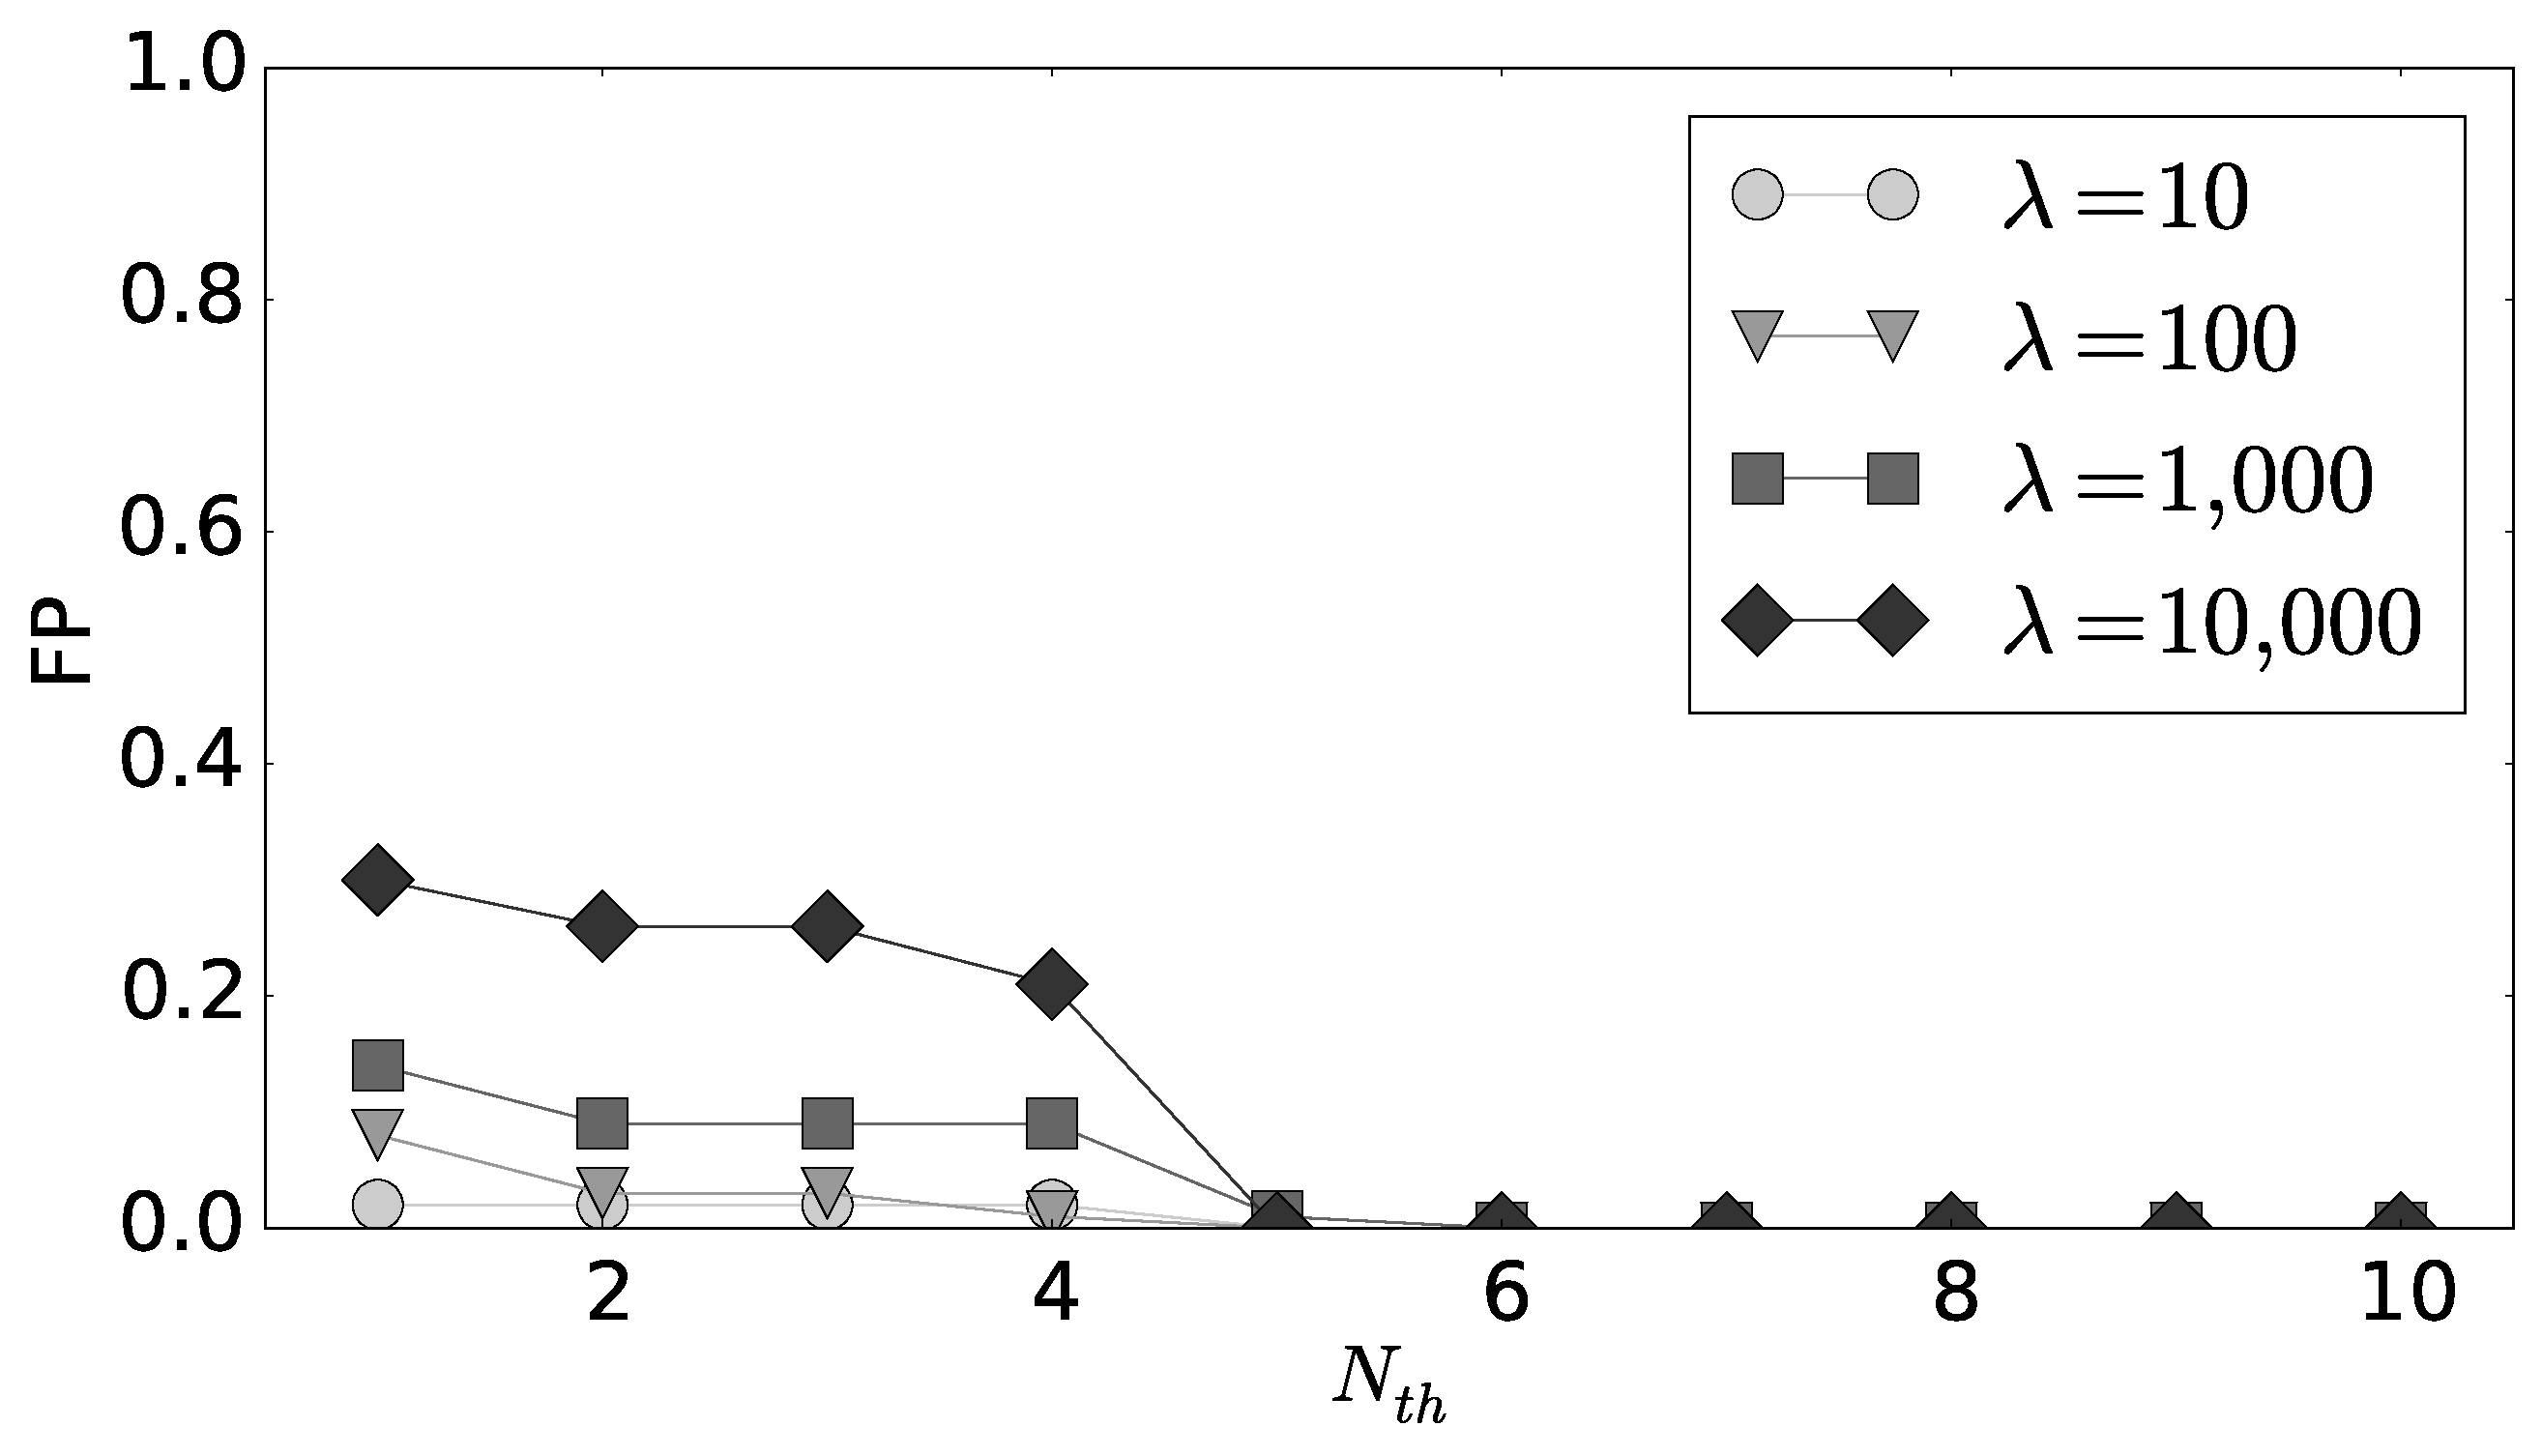
\includegraphics[clip, width=3.4in]{./image/globalTPFP/globalFP_node1000.eps}
      \caption{FP of global detection server when the number of ASes is 1,000.}
      \label{fig:FP of global detection server}
    \end{figure}

  \subsection{Discussion}
    We discuss about evaluation results.
    The detection accuracy of our scheme depends on the number of traceroute packets an AS receives.
    Our scheme efficiently detects the attack on ASes which receive sufficient number of traceroute packets.
    It is desirable to select ASes which can detect the attack with high accuracy as an input of the global detection server.
    Therefore we used the number of customer ASes to select such ASes and our scheme detects the attack with high accuracy using selected ASes.
      
    We evaluate our scheme with the model of traceroute packets randomly sent by legitimate users.
    However in the real Internet the traceroute packets may intensively be sent by legitimate uses.
    Therefore the simulation with the model which includes a burst traffics is needed to evaluate our scheme more precisely.
    The traceroute packets intensively sent by legitimate users will cause local detection servers to raise false alarms.
    This is because the traceroute packets intensively sent by legitimate users suddenly increase the number of traceroute packets.
    On the other hand, we think that the global detection server can distinguish such packets if the sudden increase of traceroute packets is local.
    This is because the global detection server uses the combination of local detection servers located across the network and an alarm sent by only one AS is considered as an false alarm.

  \section{Conclusion}\label{Sec:Conclusion}
    In this paper, we have proposed a detection scheme of the target link flooding attack.
    Our scheme detects the attack before a link congestion occurs.
    Instead of characteristics of a congested link and the router's link failure detection mechanism, we use a behaviour of increase of traceroute packets which is caused by the attacker's reconnaissance.
    By computer simulation, we show that our scheme can detect the attack at the detection servers located within ASes which connect to many customer ASes and receive the sufficient number of traceroute packets.
    Such accurate ASes can detect the attack independently of the number of traceroute packets sent by legitimate users.
    Moreover our scheme uses combination of accurate detection servers to eliminate the local increase of traceroute packets sent by legitimate users.
    On the real Internet topology, our scheme can detect the target link flooding attack with high TP and low FP. 

  \section*{Acknowledgment}
    This work is partly supported by the Grant in Aid for Scientific Research (No.26420369) from Ministry of Education, Sport, Science and Technology, Japan.

  \bibliographystyle{IEEEtran}
  \nocite{*}
  \bibliography{IEEEabrv}
  
\end{document}
